\documentclass{beamer}
\usetheme{metropolis}
%
%%% EU logo
% small version for upper right corner of normal pages
\pgfdeclareimage[width=12.8cm]{jrc-logo}{JRC_header}
\logo{\pgfuseimage{jrc-logo}}
\pgfdeclareimage[height=5.5mm]{footimage}{JRC_footer}
\pgfdeclareimage[width=0.5\textwidth]{title-image}{Bayer}
\titlegraphic{\pgfuseimage{title-image}}
%%% end EU logo


% NOTE: 1cm = 0.393 in = 28.346 pt;    1 pt = 1/72 in = 0.0352 cm
\setbeamersize{text margin right=3.5mm, text margin left=7.5mm}  % text margin

% colors to be used
\definecolor{text-grey}{rgb}{0.45, 0.45, 0.45} % grey text on white background
\definecolor{bg-grey}{rgb}{0.66, 0.65, 0.60} % grey background (for white text)
\definecolor{eu-blue}{RGB}{55, 172, 222} % blue text
\definecolor{drk-blue}{RGB}{0, 51, 102} % blue text
\definecolor{fu-blue}{RGB}{0, 51, 102} % blue text
\definecolor{fu-green}{RGB}{153, 204, 0} % green text
\definecolor{fu-red}{RGB}{204, 0, 0} % red text (used by \alert)

% switch off the sidebars
\setbeamersize{sidebar width left=0cm, sidebar width right=0mm}
\setbeamertemplate{sidebar right}{}
\setbeamertemplate{sidebar left}{}
\setbeamertemplate{navigation symbols}{}%remove navigation symbols

% frame title
\setbeamertemplate{frametitle}{%
    \vskip-5pt \color{drk-blue}\Large%
    \begin{minipage}[b][23pt]{\textwidth}%
    \flushleft \textbf{\insertframetitle}%
    \end{minipage}%
}

%%% title page
\setbeamertemplate{title page}{
% set the title
\parbox[top][2.8cm][c]{\textwidth}{\begin{center} \color{drk-blue}\Large \textbf{\inserttitle}  \\ \vspace{10pt} \small \insertsubtitle \end{center}}

% title image of the presentation
\begin{minipage}{0.5\textwidth}
\flushleft
%\hspace{-7.5mm}
\inserttitlegraphic
\end{minipage}
% Author info
\hspace{0.5cm}
\begin{minipage}{0.4\textwidth}
{\flushleft \color{black} \textbf{\insertauthor} \\ \vspace{15pt} \insertinstitute }
\end{minipage}
}
%%% end title page

%%% colors
\usecolortheme{lily}
\setbeamercolor*{normal text}{fg=drk-blue, bg=white}
\setbeamercolor*{alerted text}{fg=fu-red}
\setbeamercolor*{example text}{fg=fu-green}
\setbeamercolor*{structure}{fg=fu-blue}

\setbeamercolor*{block title}{fg=white,bg=black!50}
\setbeamercolor*{block title alerted}{fg=white,bg=black!50}
\setbeamercolor*{block title example}{fg=white,bg=black!50}

\setbeamercolor*{block body}{bg=black!10}
\setbeamercolor*{block body alerted}{bg=black!10}
\setbeamercolor*{block body example}{bg=black!10}

\setbeamercolor{item}{fg=eu-blue}
%%% end colors

\setbeamertemplate{itemize items}[circle] % if you want a ball
\setbeamertemplate{itemize subitem}[circle] % if you want a circle
\setbeamertemplate{itemize subsubitem}[circle] % if you want a triangle

%%% headline
\setbeamertemplate{headline}{
\insertlogo
}
%%% end headline

%%% footline
\newcommand{\footlinetext}{\insertdate}
\setbeamertemplate{footline}{
\begin{minipage}{58mm}
 \color{drk-blue} \hspace{7.5mm} %European Commission
\end{minipage}
\hspace{0.1mm} 
\begin{minipage}{8.5mm}
 \pgfuseimage{footimage}
\end{minipage}
\hspace{0.1mm}
\begin{minipage}{50mm}
 \color{drk-blue} 
 \flushright \insertframenumber \,/\,\inserttotalframenumber
\end{minipage}
}
%%% end footline

%%% code to remove headline
\makeatletter
    \newenvironment{withoutheadline}{
        \setbeamertemplate{headline}[default]
        \def\beamer@entrycode{\vspace*{-\headheight}}
    }{}
\makeatother
%%% end code to remove headline

\usepackage[english]{babel}
\usepackage{graphbox,graphicx}
\usepackage{url}
\usepackage{amsmath}
\usepackage{pifont}
\usepackage[T1]{fontenc}
\usepackage[font=small,labelfont=bf]{caption}
\usepackage{color}
\usepackage{booktabs}
\fontfamily{verdana}\selectfont
\setlength{\unitlength}{\textwidth}  % measure in textwidths
\setbeamercolor{item}{fg=black}
\setbeamertemplate{itemize items}[triangle] % if you want a ball
\setbeamertemplate{itemize subitem}[triangle] % if you want a circle
\setbeamertemplate{itemize subsubitem}[triangle] % if you want a triangle
\newcommand{\code}[1]{{\texttt{#1}}}

%************ Title & Author ***********************
\title{Running MSE analysis with the a4a platform}
\subtitle{[subtitle]}
\author{[author] \\ \normalfont {\scriptsize \href{mailto:jdoe@doe.com}{<[email]>}}}
\institute{[affiliation]}
\subject{Fisheries Management}

\begin{document}

%*******************************************
\begin{frame}
\titlepage

\end{frame}

%*******************************************
\begin{frame}
\frametitle{Modular MSE}

\Large \centering What is a modular MSE and how does it help ?

\vspace{1cm}

(hint: think of lego !) 

\end{frame}

%*******************************************
\begin{frame}
\frametitle{The management cycle}

\centering
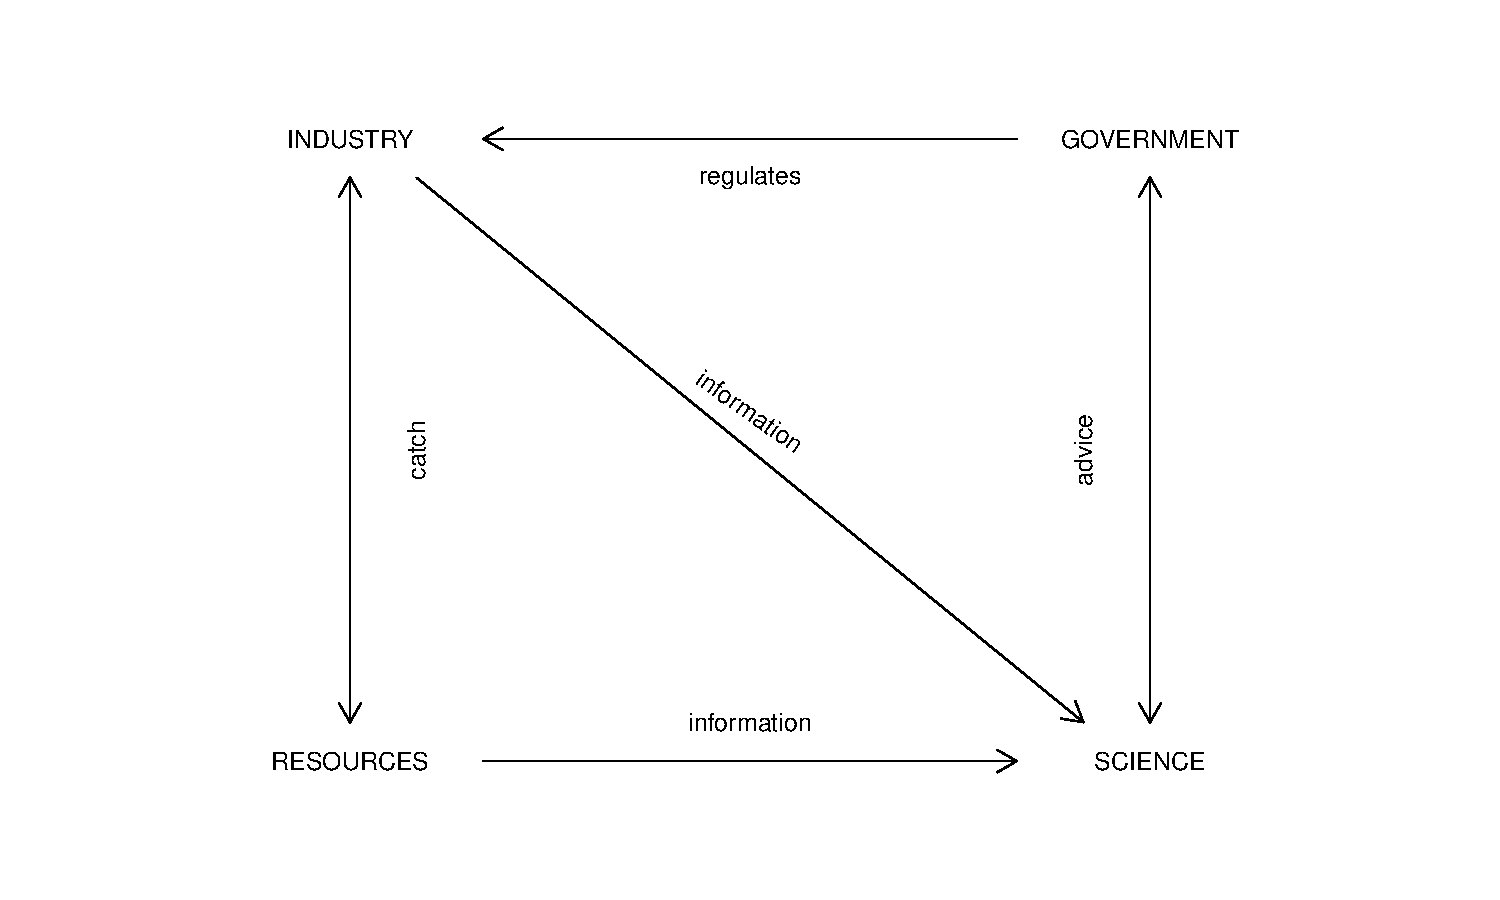
\includegraphics[height=0.8\textheight]{managementCycle2}

\end{frame}

%*******************************************
\begin{frame}
\frametitle{MSE overview}
	
\begin{center}
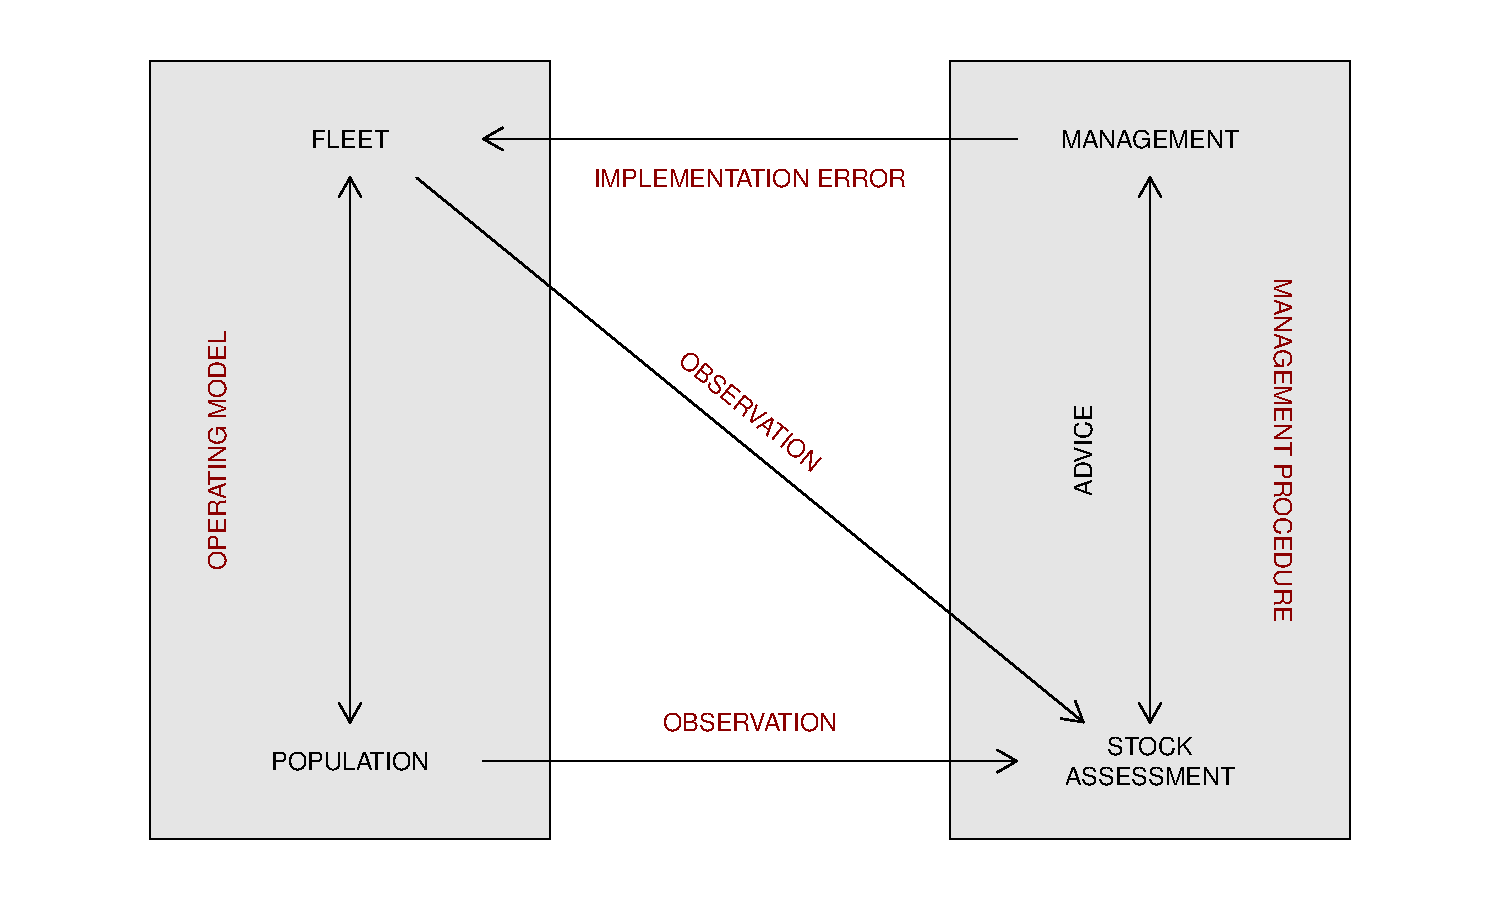
\includegraphics[height=0.8\textheight]{mse}
\end{center}
	
\end{frame}

%*******************************************
\begin{frame}
\frametitle{Generalizing and modularizing the a4a MSE}
	
\begin{center}
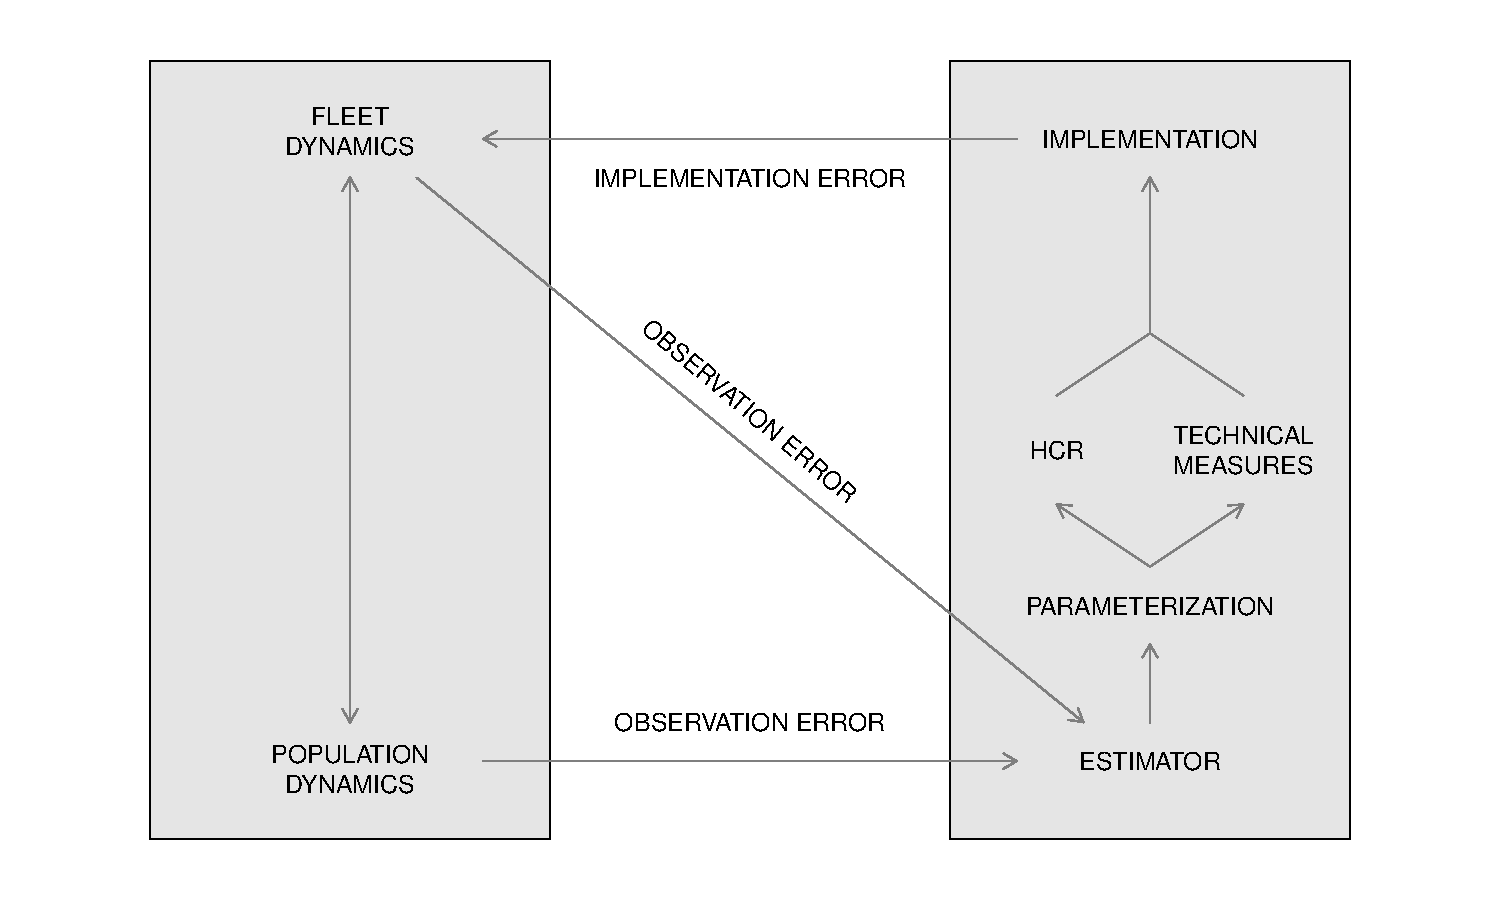
\includegraphics[height=0.8\textheight]{msea4a2}
\end{center}
	
\end{frame}

%*******************************************
\begin{frame}
\frametitle{Timeline}
	
\begin{center}
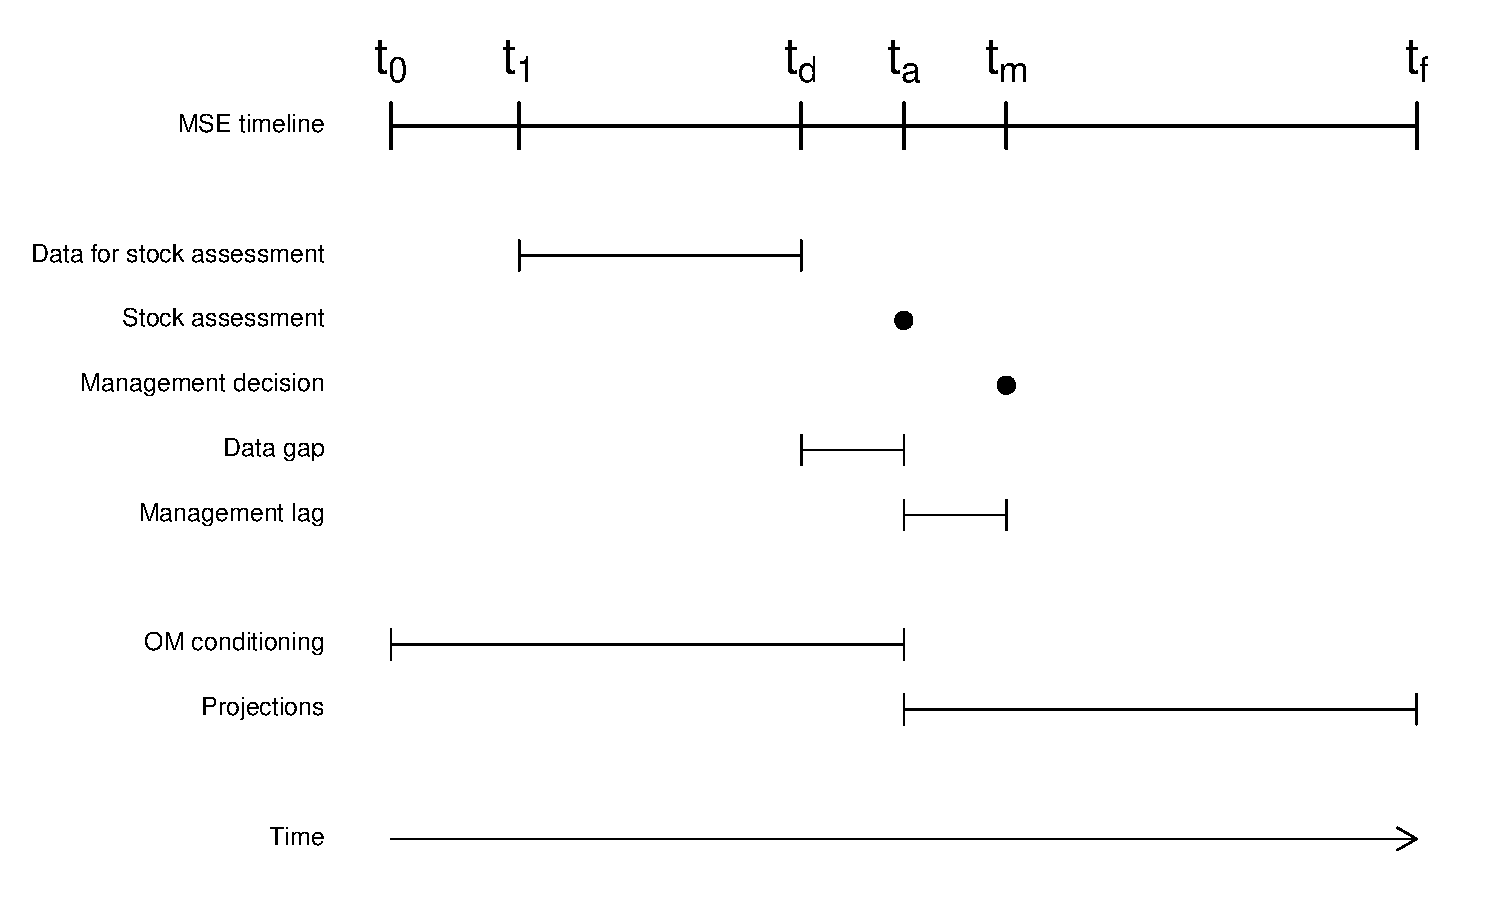
\includegraphics[height=0.8\textheight]{timeline}
\end{center}
	
\end{frame}


%*******************************************
\begin{frame}
\frametitle{Advantages of abstraction}

\footnotesize

\begin{table}
	\begin{tabular}{l|c|c}
		\hline 
		Module	& Data rich & Data limited \\ 
		\hline 
		\hline 
		Observation model	&  catch-at-age, survey & catch length frequencies \\ 
    & & \\
		%\addlinespace[.2cm]
		Estimator	& statistical catch-at-age &  $\bar{L}_{current}$ \\ 
    & & \\
		%\addlinespace[.2cm]
		Parametrization	& $F_{MSY}$ &  $L_{opt}$ \\ 
    & & \\
		%\addlinespace[.2cm]
		HCR	& $F_{future}=F_{MSY}$ & $\delta_{future}=\frac{\bar{L}_{current}}{L_{opt}}$ \\ 
    & & \\
		%\addlinespace[.2cm]
		Technical measures	& [MPA (changes F@age)] & [MPA (changes $\bar{L}_{catch}$)] \\ 
    & & \\
		%\addlinespace[.2cm]
		Implementation	& $TAC=f(C_{past}|HCR)$ & $TAC=f(C_{past} \lor E_{past}|HCR)$ \\ 
    & & \\
		%\addlinespace[.2cm]
		Implementation error	& Uncertainty in catch & Uncertainty in catch \\ 
		\hline 
	\end{tabular} 
	
	\caption{Comparative example of full feedback and data limited MSEs}
\end{table}

\end{frame}

%*******************************************
\begin{frame}
\frametitle{Comments about modular approach}

\Large

\begin{dinglist}{212}
  \item Break large complex system into simpler parts,
	\item Make it simpler to implement and share methods,
	\item Reduces the current workload,
	\item Improves readability, replicability, etc, 
	\item Improves communication !
\end{dinglist}

\end{frame}

\end{document}
